\section{Class diagram}

\todo[inline]{Relire}

The following class diagram is a schematic representation of the various objects used in our implementation and their relations. In this section we will do a short explanation of each classes and their aims.\newline

First, the participant class, this class is used to represent player in the application. Once an account as been created on the website, a participant class will be created with it to store the player's data. This class also extends the default User class of Django which allows us to easily safely save password and username in database through encryption.\newline

If a player has not yet validated his mail address, an UserInWaitOfActivation class will also be created. This class contains the key which will allow them to validate their email as well as the date of their account creation. If an account has not been validated for seven days it will thus be deleted as it probably never will.\newline

For staff member, which are also represented through the participant class, the class LogActivity will also be used, storing the data of some of the various operation that they can effectuate on the website. \newline

Similarly to the participant class, the court class is used to represent courts and contain their information. As you can see, both classes posses a latitude and longitude attribute which allows us to store their relative emplacement. That information can then be used to reduce participant's travel distance during the tournament creation, by selecting court which accommodate a maximum of participant. \newline

As you can see the court class is also linked to three small classes, courtSurface, courtState and courtType, which serve to alleviate the load on the database by reducing data replication. The participant class is similarly linked to a small ranking class which serve the same purpose. \newline

The pair class is used to store pairs data in the application. Each pair being composed of two participant and of various other attribute as the list of extras that they chooses to pay for (through the Extra class) and if they have already payed at all. \newline

This comes the need of the Extra class which allows us to store the data relative to and extra such as it's price, name and some commentary explaining their content.\newline

The Tournoi class is used along with other classes to store all data relative to a given tournament; It is inked to three important classes that help store it's data.

First the tournoiCategorie class which stores the name and rules allowing to participate to the tournament. The rules allowing for automatic tournament selection at pair creation. 
The tournoiTitle class holds a description of the tournament, the gender both player should have to participate and the information regarding the day the tournament will be on.
Finally, the InfoTournoi class holds other important information regarding tournament such as the price or the results of the tournament once it is finished.

Two other classes are also necessary to the tournament organisation. Namely the Poule classes which each hold the data regarding a poule composed of pairs and the Arbre class which hold information regarding knock off tournament.\newline

The poule class holds information such has who is the poule leader or on which court it will take place. It is linked to a Poule status class which hold the name of the poule, again to alleviate the load on the database in case many poule had the same, and a Score class which hold the result of a confrontation between two pairs.\newline

The arbre class stores the data relative to a knock of tournament and the court it will take place on. Allowing us to store and manipulate the data.\newline

And finally the Resultats class holds data regarding the result of a tournament such as the winners and finalists. \newline

\begin{figure}[!ht]
	\centering
	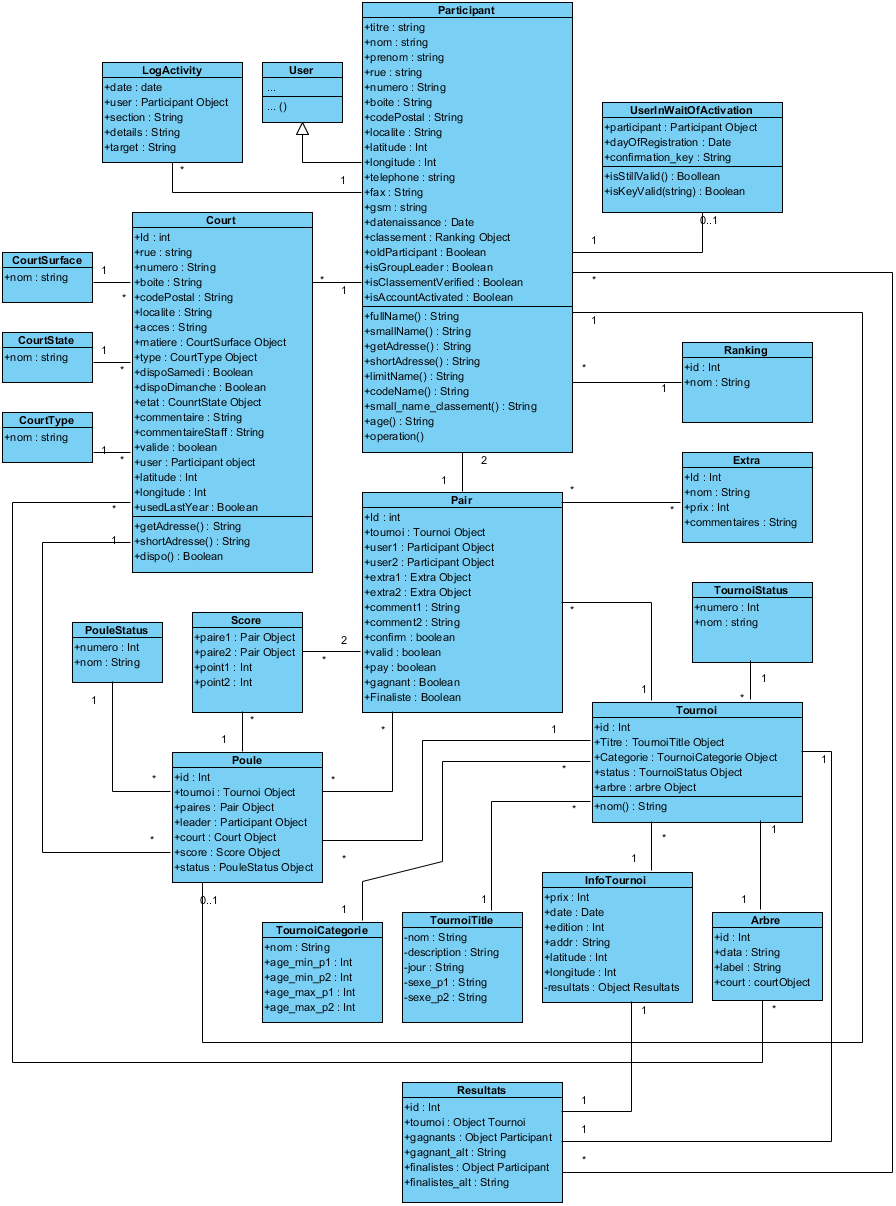
\includegraphics[width=1\linewidth]{class_dia.png}
	\caption{Class diagram of our current implementation}
	\label{fig:length_eight_mouse}
\end{figure}
\FloatBarrier